% Created 2023-10-18 Wed 23:48
% Intended LaTeX compiler: pdflatex
\documentclass[12pt, a4paper]{article}
\usepackage[utf8]{inputenc}
\usepackage[T1]{fontenc}
\usepackage{graphicx}
\usepackage{longtable}
\usepackage{wrapfig}
\usepackage{rotating}
\usepackage[normalem]{ulem}
\usepackage{amsmath}
\usepackage{amssymb}
\usepackage{capt-of}
\usepackage{hyperref}
\usepackage{placeins}
\usepackage{gensymb}
\usepackage[letterpaper]{geometry}
\geometry{top=1.0in, bottom=1.0in, left=1.0in, right=1.0in}
\usepackage{rotating}
\usepackage{graphicx}
\usepackage{pgfplots}
\usepackage{filecontents}
\usepackage{tikz}
\usepackage{fancyhdr}
\usepackage{enumitem}
\pagestyle{fancy}
\usepackage{listings}
\usepackage{matlab-prettifier}
\usepackage{subcaption}
\lhead{}
\chead{}
\rhead{Johnson \thepage}
\lfoot{}
\cfoot{}
\rfoot{}
\renewcommand{\headrulewidth}{0pt}
\renewcommand{\footrulewidth}{0pt}
\setlength\headsep{0.333in}
\newcommand{\bibent}{\noindent \hangindent 40pt}
\newenvironment{workscited}{\newpage \begin{center} Works Cited \end{center}}{\newpage }
\graphicspath{ {./attachments/} }
\author{Christian}
\date{\today}
\title{}
\hypersetup{
 pdfauthor={Christian},
 pdftitle={},
 pdfkeywords={},
 pdfsubject={},
 pdfcreator={Emacs 28.2.50 (Org mode 9.7-pre)}, 
 pdflang={English}}
\begin{document}

\begin{document}
\begin{flushleft}
Christian Johnson\\
\vspace{2mm}Dr. Richard Hartnett\\
\vspace{2mm}Linear Circuits\\
\vspace{2mm}October 16 2023\\
\vspace{4mm}\begin{center}
Lab 3 Report
\end{center}
\vspace{1mm}\setlength{\parindent}{0.5in}


\begin{abstract}
The purpose of this lab, entitled a study of real world op-amps, is to learn about real world operational amplifier characteristics, as compared to ideal operational amplifier assumptions. This report presents the results of measurements conducted on the 741 op-amp using laboratory equipment, matlab, and multisim. More specifically, our investigations focused on parameters such as slew rate, gain bandwidth product, input bias current, and open loop output impedance for inverting amplifier configurations. We show that, in an inverting configuration, the 741 op-amp behaves like an ideal op-amp provided the input signal frequency and amplitude are well within the gain bandwidth product and slew rate limitations for the device.

Furthermore, we conducted a comparative analysis of theoretical open and closed loop magnitude response plots, underscoring the relative consistency between experimental and predicted results.

In conclusion, the results of this study provide invaluable insight into the practical behavio of the LM741 operational amplifier. The alignment between laboratory findings and theoretical expectations emphasizes the importance of considering real-world operational amplifier characteristics in engineering decisions. These insights are crucial for informed decision making when selecting and designing operational amplifiers and the circuits that utilise them.
\end{abstract}
\section{Introduction}
\label{sec:orge24290b}

Throughout this report, there are several reoccurring concepts that are important to understand before moving forward. In general, operational amplifiers (or op-amps for short) are voltage amplifying devices. They have two input terminals, typically referred to as the inverting (-) and non-inverting (+) terminals, and are intended for use with components like resistors, capacitors, and inductors arranged in different configurations in order to produce different amplifications [2]. These op-amps have certain inherent properties that determine their efficiency and suitability for certain situations. Gain is the static multiplier, where an op-amps output voltage is the input multiplied by gain. Gain bandwidth product is this gain value multiplied by the bandwidth, or the op-amps effective frequency range. This value typically depends on the load resistor, meaning that gain and bandwidth must be adjusted to achieve a desirable result. Slew rate describes the maximum rate at which the voltage can change, typically measured in volts per microsecond. Input offset voltage refers to the input voltage needed to produce a zero volt output. This is particularly relevant to open-loop op-amps, which describes an op-amp configuration where there is no feedback between the output and input [3]. Conversely, closed loop op-amp configurations feature a direct connection between output voltage and input voltage, typically over some feedback component. In almost every op-amp, there will be some DC current in the input terminals. Input Bias Current describes the average of the two currents, and Input Offset Current is the difference of the two. These values are particularly important when dealing with high impedance components, since even small currents can cause a significant impact.
\section{Theory}
\label{sec:org93ab4e8}

Having defined these fundamental op-amp parameters, it is important to now recognize the difference between ideal and non-ideal "real world" op-amps. Many of the formulas and methods used to find these values make certain assumptions that may not always be true. Because of this, there are often differences between the expected value and what is actually shown in the results.Theoretical models offer an initial understanding of these parameters, allowing us to predict how op-amps should behave in idealized scenarios. However, when employing real-world op-amps, it is crucial to recognize that theoretical expectations are often met with imperfections and inconsistancies. This section explores the theoretical calculations that provide the basis for further experimentation. Calculating theoretical values allows for a better understanding of real world data, and provides a comparison point for any conclusions drawn later.

When examining operational amplifiers, theoretical calculations are taken under the assumptions of an ideal op amp. Under such conditions, open-loop gain and input impedance are assumed to be infinite, and the output impedance is assumed to be 0. Because of this high input impedance, there will be next to no current flowing through the input terminals of the op amp, and the voltage difference between these two terminals is assumed to be 0.

Most op amp analysis involves finding the Gain Bandwidth Product, Input Offset Voltage, Input Bias Current, Input Offset Current and Slew Rate. Typically, these values are easiest to find through experimentation, but there are general ranges for each based on the op amp used. For an LM741, one should expect a Slew Rate between \(0.5V/\mu s\) and \(0.8V/\mu s\), an Input Offset Voltage of about \(1mV\), Input Bias Current around \(80nA\) and Input Offset Current near \(10nA\).

One of the most important things to understand when using an operational amplifier is how it will respond to input under different conditions. One method for accomplishing this, is to use Multisim to simulate a range of inputs to theoretical circuits in order to model the op amps response. The transfer function of an op amp is defined to be the open loop frequency response, but since op amps can become unstable when outside of a larger circuit, it is simpler to construct a closed loop circuit and measure the open loop response within this larger circuit.
\begin{figure}[htb]
\centering
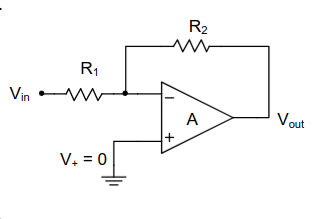
\includegraphics[width=0.3\textwidth]{PartBCircuit.png}
\caption{Measuring Open Loop Response}
\end{figure}
This figure illustrates an inverting amplifier. Assuming resistor values of \(100k\Omega\) and \(1k\Omega\), the amplifier has a gain of -100, which means that any input signals will decrease by a factor of 100. The open loop response of this circuit should demonstrate a relatively high magnitude response near 1 Hz, decreasing rapidly as it approaches 500 kHz. This range comes from the op amps inherent Gain Bandwidth Product. In contrast, the closed loop response for the same circuit demonstrates a much lower magnitude response, since the feedback components in the circuit serve to limit the op amps output. Furthermore, modifying the resistor values in the circuit to decrease the gain will derease the magnitude response even more. This relationship is shown in figure 2, where all 3 of these curves are overlaid.
\begin{figure}[htb]
\centering
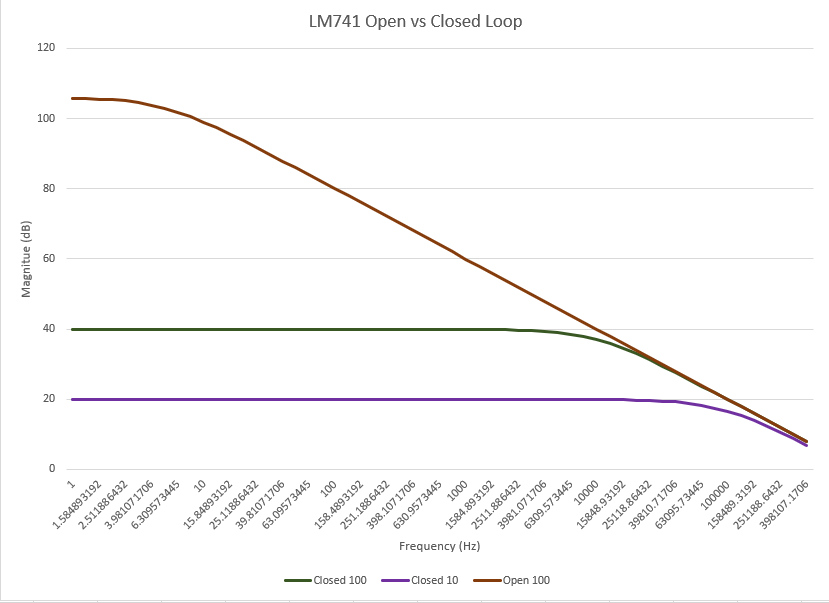
\includegraphics[width=0.5\textwidth]{PartBOverlay.png}
\caption{Magnitude Response from 1 Hz to 500 kHz}
\end{figure}
In this figure, it becomes clear that the open loop magnitude response is highest at low frequencies. The closed loop response is almost half that of the open loop, and the change in resistance lowers it by another approximate factor of two.

Matlab is another common tool that can be used to analyze amplifier circuits. It is useful for creating plots of complex design functions and comparing them among each other. Given two inverting amplifier circuits with gains of -10 and -100, it is possible to use Matlab to calculate and plot the expected representations for their respective frequency responses. These plots should look similar to those produced earlier in Multisim, since the premise is the same. The graphs below show the theoretical frequency response for these two circuits.

\begin{figure}[htb]
\centering
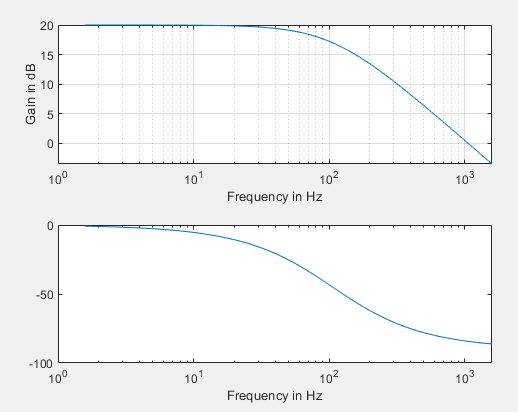
\includegraphics[width=0.4\textwidth]{PartD10.png}
\caption{Frequency Response - Gain = 10}
\end{figure}
\begin{figure}[htb]
\centering
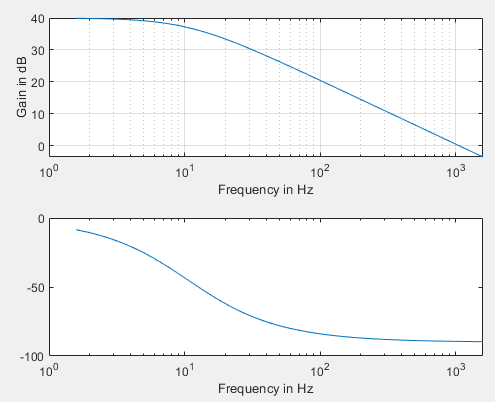
\includegraphics[width=0.4\textwidth]{PartD100.png}
\caption{Frequency Response - Gain = 100}
\end{figure}

In these graphs, the magntude plot is similar to those found earlier with multisim. This is to be expected, despite the slight differences in the circuits, since both function as low pass filters with relatively proportional characteristics. 
\section{Methodology}
\label{sec:org26bcdd6}

In this section, we outline the procedures and methods for measuring operational amplifier characteristics, essential for understanding their practical behavior and deviations from ideal models.
\subsection{Part A}
\label{sec:orga16fb43}
Part A of this lab involves calculating slew rate, input offset voltage, input offset current, and input bias current for the op amp in Figure 5.
\begin{figure}[htb]
\centering
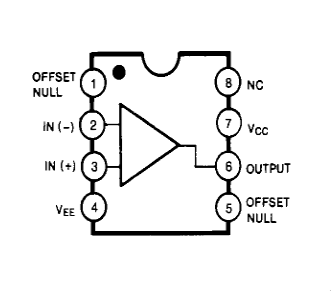
\includegraphics[width=0.4\textwidth]{LM741Pinout.png}
\caption{LM741 Operational Amplifier}
\end{figure}
In order to properly measure these characteristics, it was necessary to construct several different circuits and measure the input and output across the op amp in various situations. Input offset voltage, defined earlier as the input voltage required to produce a zero volt output, can be found by connecting the output pin to the op amps non-inverting pin and wiring the inverting pin to ground as shown in Figure 6 below.
\begin{figure}[htb]
\centering
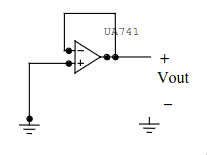
\includegraphics[width=0.2\textwidth]{InputOffset.png}
\caption{Measuring Input Offset Voltage}
\end{figure}

We use this configuration because in this state, output voltage and input voltage are equal. Ideally, when there are no feedback components and no input voltage, the output would also be zero. Since this is not an ideal situation however, there will be a small amount of output. We measure that output at \(V_{out}\) and we can treat this value as our offset voltage. This can be summarized in equation 1.
\begin{equation}
V_{\text{OS}} = V_{\text{out}}
\end{equation}
Next, to find the input bias current and input offset current, we use variations of the circuit in Figure 2. The goal is to individually find the current in each terminal, and then combine those into the necessary values. Figure 7 shows the circuit needed to find current in the inverting terminal, and Figure 8 shows the circuit necessary for the non-inverting terminal.
\begin{figure}[htb]
\centering
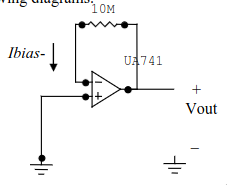
\includegraphics[width=0.3\textwidth]{InputBiasNeg.png}
\caption{Current in Inverting Terminal}
\end{figure}
\begin{figure}[htb]
\centering
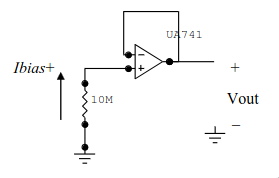
\includegraphics[width=0.3\textwidth]{InputBiasPos.png}
\caption{Current in Non-Inverting Terminal}
\end{figure}

Using these circuits, finding the current components becomes trivial, illustrated by the following formulae.
\begin{equation}
Ibias(-)=\frac{V_{\text{out}}\text{(fig. 3)}}{10M\Omega}
\end{equation}
\begin{equation}
Ibias(+)=-\frac{V_{\text{out}}(\text{fig. 4})}{10M\Omega}
\end{equation}
These components can then be combined to find input bias current and input offset current.
\begin{equation}
BC=\frac{Ibias(-)*Ibias(+)}{2}
\end{equation}
\begin{equation}
OC=Ibias(-)-Ibias(+)
\end{equation}
Finally, in order to find slew rate, the maximum rate at which an op amps voltage can change per unit time, it is necessary to understand how to induce rapid change in an op amp. The best way to make output change rapidly is to change input rapidly, and a square wave is the simplest way to vary input. Using a square wave as input will produce a rapid change in the output, which can then be measured with the Digital Signal Analyzer. Measuring the output voltage will produce a curve, and the slope of that curve represents the slew rate. This is due to the fact that output voltage divided by input voltage will produce the rate at which the output changes.
\subsection{Part B}
\label{sec:org60100e2}

Part B consists primarily of constructing circuits in multisim. Figure 1 shows the initial circuit, meant to be an inverting amplifier with a gain of -100 using a \(100k\Omega\) resistor fo r\(R_{2}\). Given the following equation for gain of an inverting amplifier, we calculated \(R_{1}\) as 1 Ohm. 
\begin{equation}
\frac{V_{out}}{V_{in}} = -\frac{R_{f}}{R_{in}}
\end{equation}

Using multisim, we generated the open loop magnitude response (\(\frac{V_{out}}{V_{-}}\)) from 1Hz to 500kHz. From this graph, we were able to calculate gain bandwidth product using equation 7.
\begin{equation}
\text{Gain Bandwidth Product}=\text{Gain}*\text{Freq.}
\end{equation}
Next, we switched our simulation to calculate the closed loop magnitude response (\(\frac{V_{out}}{V_{in}}\)) over the same range. Finally, switching \(R_{2}\) to \(10k\Omega\) in order to produce a gain of -10, we are left with the data shown in figure 2. 
\subsection{Part C}
\label{sec:orgf2af46a}

Part C was the most measurement focused section of the lab, focusing primarily on using the Digital Signal Analyzer (DSA) and matlab to examine physical circuits. We began by constructing the circuit shown in figure 9.
\begin{figure}[htb]
\centering
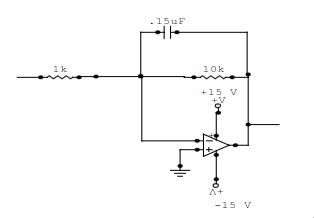
\includegraphics[width=0.4\textwidth]{PartCCircuit.png}
\caption{Part C Circuit}
\end{figure}

Using the DSA, we measured and plotted the open loop response (\(\frac{V_{out}}{V_{-}}\)). Using these graphs, with gain on the Y axis and frequency on the X axis, we are able to calculate the actual value for GBP using the following formulae.
\begin{equation}
\text{Linear Gain} = 10^{\frac{Gain(dB)}{20}}
\end{equation}
\begin{equation}
GBP = \text{Freq.} * \text{Linear Gain}
\end{equation}

Moving on from this circuit, we were tasked with constructing an amplifier circuit with a gain of -10. This was simply a basic inverting amplifier (shown in figure 1) with \(R_{f} = 10k\Omega\) and \(R_{i} = 1k\Omega\). Using the DSA we plotted the frequency response (\(\frac{V_{out}}{V_{in}}\)). This produces magnitude and phase plots, which we were able to transfer to matlab. We repeated this process for an amplifier with gain of -100, simply using new resistor values, \(R_{f} = 100k\Omega\) and \(R_{i} = 1k\Omega\). Finally, we connected a \(200\Omega\) resistor to the existing load resistor. Repeating the same process from before, we plotted this in the DSA and transferred the data to Matlab.
\subsection{Part D}
\label{sec:org3b766ed}

Part D involved very little actual data collection. Instead, we were meant to theoretically calculate the transfer function, and plot the result using Matlab. Overlaying the experimental graph of magnitude response for a closed loop gain of both 10 and 100 with this Matlab plot and the results from the earlier Multisim simulation produces a reasonable comparison for ideal and experimental data for these values.

\begin{figure}[htb]
\centering
\begin{subfigure}{0.4\textwidth}
\centering

\includegraphics[width=\linewidth]{PartDCircuit10.png}
\caption{10\Omega}
\end{subfigure}
\begin{subfigure}{0.4\textwidth}
\centering

\includegraphics[width=\linewidth]{PartDCircuit100.png}
\caption{100\Omega}
\end{subfigure}
\caption{Amplifier Circuits}
\end{figure}
The circuits in figure 10 provided the basis to derive the block diagrams in figure 11.
\begin{figure}[htb]
\centering
\begin{subfigure}{0.4\textwidth}
\centering
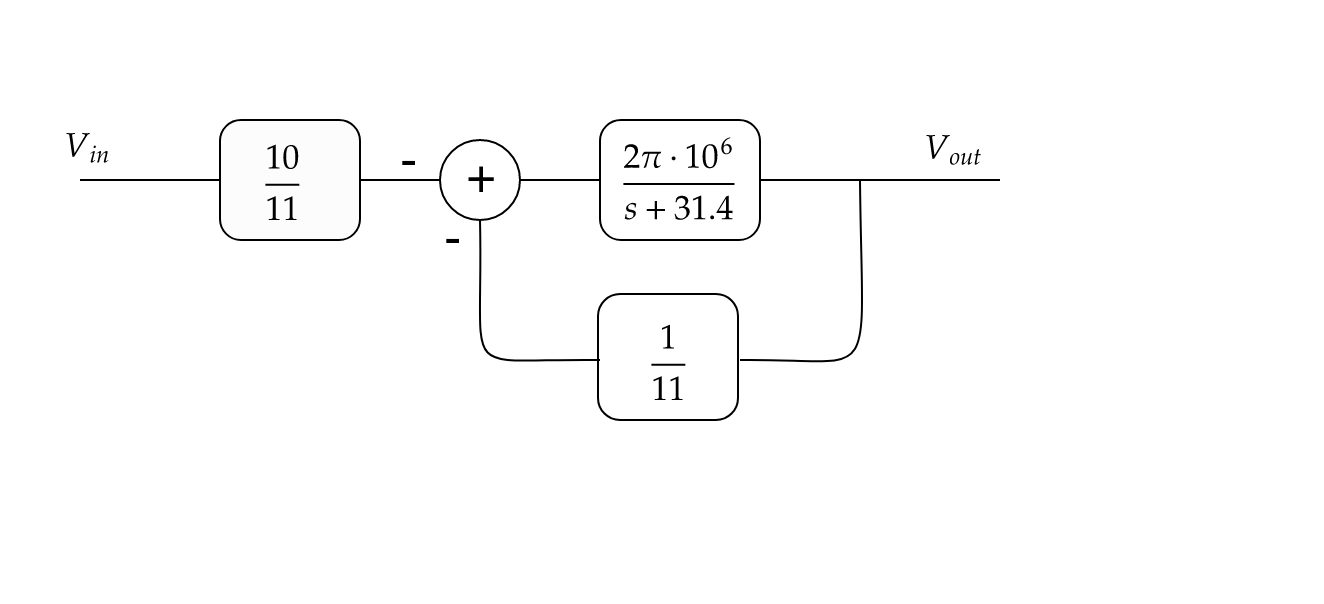
\includegraphics[width=\linewidth]{PartDBlock10.png}
\caption{10\Omega}
\end{subfigure}
\begin{subfigure}{0.4\textwidth}
\centering
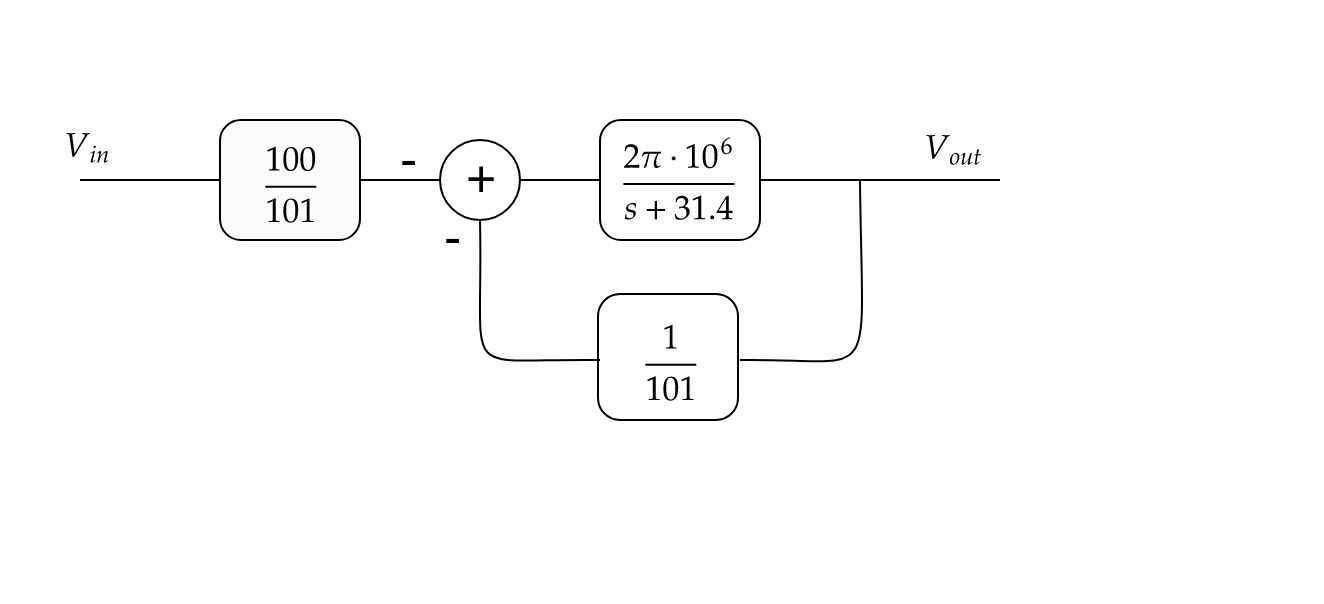
\includegraphics[width=\linewidth]{PartDBlock100.png}
\caption{100\Omega}
\end{subfigure}
\caption{Block Diagrams for Amplifier Circuits}
\end{figure}
From the block diagrams in figure 11, we are able to derive the transfer functions in equations 10 and 11.
\begin{equation}
H(s) = \frac{-(\frac{100}{101})\frac{2\pi*10^6}{s+31.4}}{1+(\frac{1}{100})\frac{2\pi*10^6}{s+31.4}}
\end{equation}
\begin{equation}
H(s) = \frac{-(\frac{10}{11})\frac{2\pi*10^6}{s+31.4}}{1+(\frac{1}{10})\frac{2\pi*10^6}{s+31.4}}
\end{equation}
\section{Results and Analysis}
\label{sec:orgdd83c00}
\subsection{Part A}
\label{sec:org28eaba0}

\begin{figure}[htb]
\centering
\begin{tabular}{|l|l|l|}
\hline
Dimension & Expected Values & Experimental Values \\
\hline
Slew Rate & 0.5 $V/\mu s$ to 0.8 $V/\mu s$ & 0.71 $V/\mu s$ \\
Input Offset Voltage & 1 mV & 0.43 mV \\
Input Offset Current & 80 nA & 1 nA \\
Input Bias Current & 10 nA & 1 nA \\
\hline
\end{tabular}
\caption{Comparison of Expected and Experimental Values}
\end{figure}
The table shown above depicts the values obtained in part A. The LM741 op amp used to generate these results was within the expected range for most values, performing slightly better than expected in some cases.
\subsection{Part B}
\label{sec:org503ca3d}

Part B consisted primarily of trials inside Multisim in order to evaluate the LM741 op amp. Measuring the LM741's magnitude response provides an interesting assessment of the op amps performance over a given range of values, but without any values to compare against this data can be difficult to contextualize. Shown below is the magnitude response for both an LM741 and an LM318 from 1 Hz to 500 kHz.
\begin{figure}[htb]
\centering
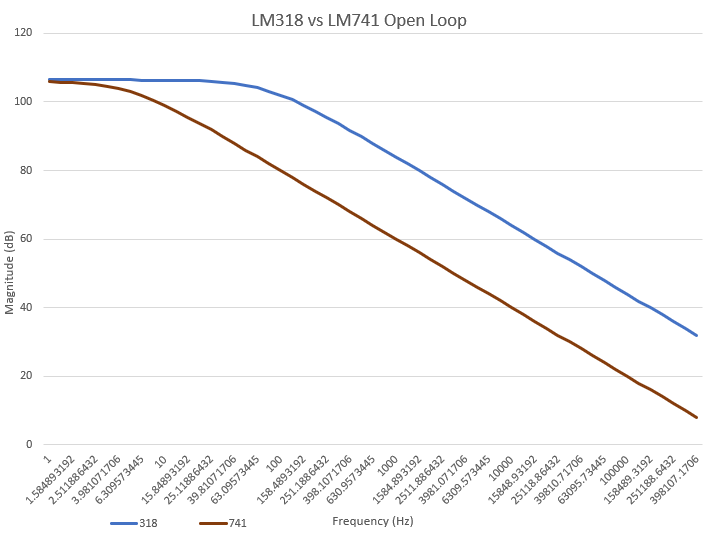
\includegraphics[width=0.5\textwidth]{PartB318v741.png}
\caption{Magnitude Response: LM741 vs. LM318}
\end{figure}
This graph shows the 318's magnitude beginning to decrease slightly after the 741, indicating that the 318 and 741 perform similarly, but for different effective frequency ranges.
Having compared the 741's performance against other operational amplifiers, it is important to next understand how different configurations of the same op amp can perform. Shown below is a graph demonstrating the LM741's \emph{closed loop} magnitude response at a gain of -10 and -100. These curves are superimposed over the previously plotted \emph{open loop} magnitude response.
\begin{figure}[htb]
\centering
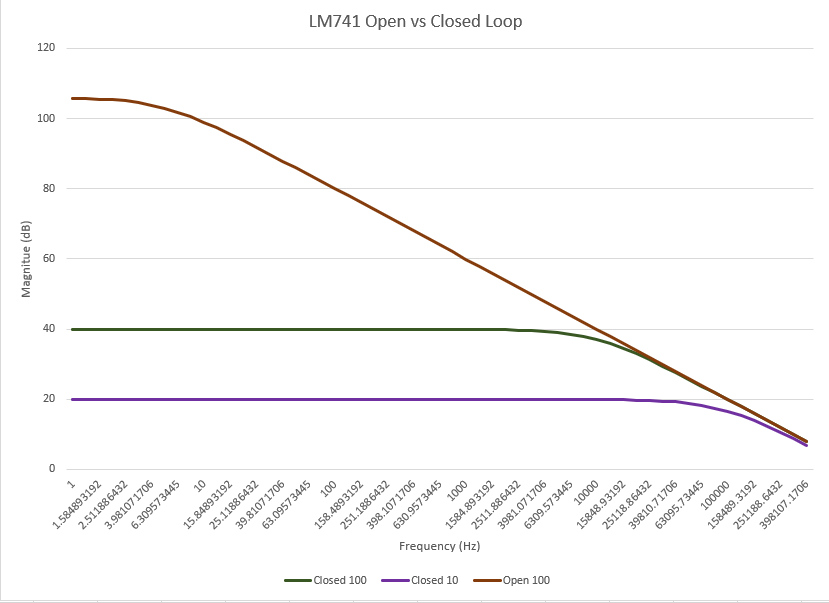
\includegraphics[width=0.5\textwidth]{PartBOverlay.png}
\caption{Magnitude Response: LM741 open vs. closed loop}
\end{figure}
As discussed in the Theory section of this report, this graph shows a gradual decrease in maximum magnitude as the circuit changes from Open Loop, to Closed, then a higher resistor value.
The graph of the 741's open loop gain can be used to visualized the gain bandwidth product of the op amp. Thus, using figure 12 and equation 7, we are able to calculate the GBP at around 1 MHz or less.
\subsection{Part C}
\label{sec:orgdc66f6f}
\begin{figure}[htb]
\centering
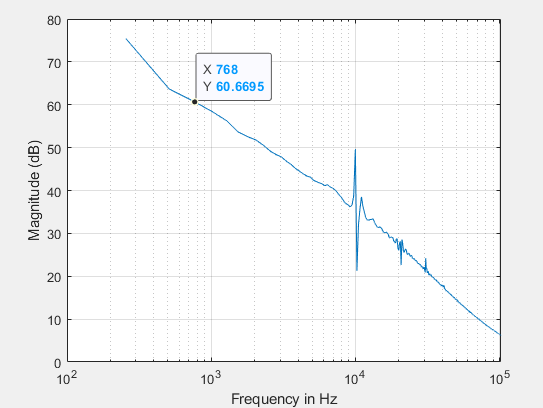
\includegraphics[width=0.5\textwidth]{PartCGBP.png}
\caption{Experimental Magnitude Response}
\end{figure}
Figure 15 shows the magnitude response of the circuit shown in figure 9. Using equation 7 again with the values shown above (\(\text{Gain}_{dB} = 60.6695\) and \(F=768 Hz\)) Gain Bandwidth Product comes to approximately 0.829 MHz. This is relatively close to the 1 MHz expected value calculated above, falling well within a reasonable margin of error to allow for human error and inaccuracies due to a non-ideal op amp.
\begin{figure}[htb]
\centering
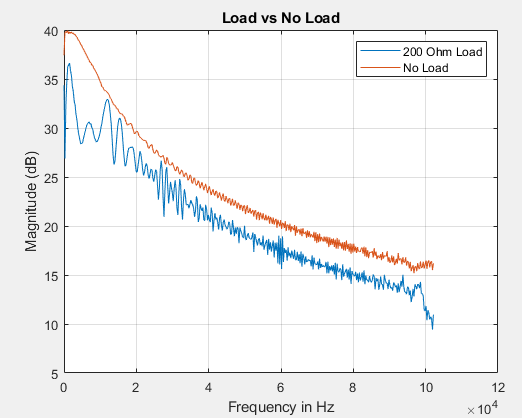
\includegraphics[width=0.5\textwidth]{PartCLoadvNoload.png}
\caption{Impact of Load on Magnitude Response}
\end{figure}
Figure 16 illustrates the magnitude response for the circuit with a closed loop gain of 100 (Orange) compared with the magnitude response with a closed loop gain of 100 and an additional \(200\Omega\) load resistance. This clearly demonstrates the impact of load resistance on magnitude response - the \(200\Omega\) circuit demonstrating markedly lower magnitude compared to the circuit with no such load.
\begin{figure}[htb]
\centering
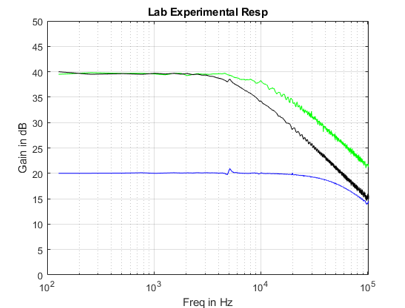
\includegraphics[width=0.5\textwidth]{PartCTriple.png}
\caption{Combined Experimental Response}
\end{figure}
Figure 17 shows the relationship between the curves shown above, alongside the response for a circuit with a closed loop gain of 10. In this graph, the circuit with the \(200\Omega\) resistor, shown in black, decreases at the quickest rate since the additional resistance forces the op amp to work harder. 
\subsection{Part D}
\label{sec:org8b75827}
\begin{figure}[htb]
\centering
\begin{subfigure}{0.4\textwidth}
    \centering
    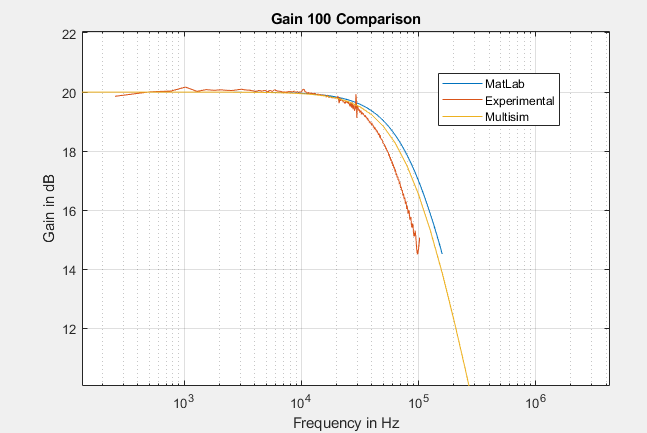
\includegraphics[width=\linewidth]{PartD10-exp.png}
    \caption{Comparison - Gain = 10}
\end{subfigure}
\begin{subfigure}{0.35\textwidth}
    \centering
    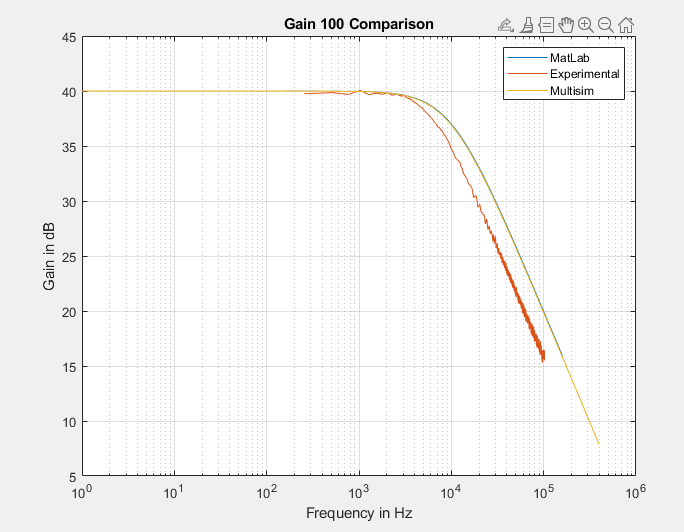
\includegraphics[width=\linewidth]{PartD100-exp.png}
    \caption{Comparison - Gain = 100}
\end{subfigure}
\caption{Comparison of Different Gains}
\end{figure}

The two graphs in figure 18 show a comparison between multisim, matlab, and experimental calculations for magnitude response when closed loop gain is either 10 or 100. In these graphs, the two theoretical calculations (Matlab and Multisim) appear relatively similar, while the experimental data appears to differ slightly. This quite clearly illustrates the difference between ideal and non-ideal op amp response - while theoretical data can provide a passable approximation for an component performance, there will always be some variation to account for in the final design. 
\section{Conclusions}
\label{sec:org2499dc6}
In this laboratory experiment, we explored the characteristics of a real world LM741 operational amplifier, comparing its performance and characteristics to what we would expect to see from an ideal op amp. We conducted a comprehensive analysis of various parameters, examining how they affect the performance of the amplifier. Experimental results for these values were consistant with expected values. Part B involved investigating the 741's magnitude response for both open and closed loop configurations. Measurements revealed a gain bandwidth product of about 1MHz, slightly below in some areas but well within the theoretical expectations. Results show the importance of choosing the correct feedback component, and the drastic impact that these components can have. Part C introduced practical circuit measurements, highlighting the impact of load resistance on magnitude response. The data gathered from the physical circuits confirmed that additonal load resistance caused a noticeable decrease in the magnitude response. Finally, in Part D, the data illustrated the disparity between the idealized theoretical predictions and real-world performance. The graph generated helped to underscore the importance of understanding and accounting for these non-ideal, real world behaviors when designing amplifier circuits.
In summary, this laboratory experiment allowed us to gain valuable insight into the behavior of the LM741 operational amplifier, and op amps in general. We observed that, while theoretical models offer a foundation for understanding the amplifier's characteristics and general performance, real world op amps exhibit variation that must be accounted for in practical applications.

\begin{workscited}
% Format: Last, F.M. TITLE. PUBLISHER, PUBDATE. PrintTYPE.
\bibitem{peterson}
[1] Peterson, Benjamin B., Richard J. Hartnett, and Keith C. Gross. \emph{Analog and Digital Filter Design}. 
\bibitem{website1}
[2] "Op-Amp Tutorial," Electronics Tutorials, \url{https://www.electronics-tutorials.ws/opamp/opamp_1.html} (Accessed: October 16, 2023).
\bibitem{website2}
[3] "Open-Loop Configuration of Op-Amp," Electronics for You, Published: October 1, 2022, \url{https://electronicsforyou.in/open-loop-configuration-of-op-amp/} (Accessed: October 16, 2023).
\bibitem{Fairchild}
[4] Fairchild Semiconductor, LM741 Single Operational Amplifier Datasheet. n.d.

\end{workscited}
\end{flushleft}


\newpage
\begin{center}
Appendices
\end{center}

\begin{lstlisting}[caption={Part D Frequency Response}, frame=single, numbers=left, style=Matlab-Pyglike]
w = logspace(1,6,1000);
b=[-2*pi*1e6]; % Other value was b = [-(10/11)*2*pi*1e6];
a = [1 2*pi*1e4]; % Other value was a = [1 2*pi*1e5];
h = freqs(b,a,w);
mag = 20*log10(abs(h));
semilogx(w/(2*pi),mag,xx,yy,closed10.x10CL1,closed.10.x10CL3);
title('Gain 100 Comparison');
legend('Matlab','Experimental','Multisim');
xlabel('Frequency in Hz');ylabel('Gain in dB');grid;
\end{lstlisting}

\begin{lstlisting}[caption={Part C Experimental Load Comparison}, frame=single, numbers=left, style=Matlab-Pyglike]
x1 = x200Ohm;
y1 = y200Ohm;
x2 = xGain100;
y2 = yGain100;

figure(3);
plot(x1, y1);
title('Load vs No Load');
xlabel('Frequency in Hz');
ylabel('Magnitude (dB)');
grid;
hold on
plot(x2, y2);
hold off
legend('200 Ohm Load','No Load');
\end{lstlisting}

\begin{lstlisting}[caption={Part D Plot}, frame=single, numbers=left, style=Matlab-Pyglike]
clear all; hold off;clf;
w=logspace(1,6,100); % generate 100 points equally spaced on a
% logarithmic axis
% from 1 rad/sec to 10,000 rad/sec
% NOTE: YOUR “b” and “a” (NUMERATOR
% and DENOMINATOR will be different!
% The next 3 lines are just provided
% to serve as an example for you
% to see how “freqs” can be used to
% calculate the frequency response for
% this sample transfer function. In this
% example, “freqs” function call returns
% the (complex) frequency response in “h”
b=[-(10/11)*2*pi*1e6]; %numerator for H(s) is -5000
a=[1 2*pi*1e5]; %denominator for H(s) is s + 500
h=freqs(b,a,w); %evaluate frequency response at those
%frequencies in the w vector
mag=20*log10(abs(h)); %Since “h” is complex, evaluate the
%MAGNITUDE (in dB)
phase=angle(h)*180/pi; %and evaluate the “angle” of “h” in degrees
subplot(2,1,1); %Do two plots (2 rows, 1 column) and
%plot in 1st window
semilogx(w/(2*pi),mag); %plot magnitude vs. frequency in Hz
xlabel('Frequency in Hz');
ylabel('Gain in dB');grid;
%subplot(2,1,2); %Do two plots (2 rows, 1 column) and
%plot in 2nd window
%semilogx(w/(2*pi),phase);
%xlabel('Frequency in Hz');
%ylabel('Phase in Degrees');grid;
\end{lstlisting}

\newpage

\end{document}
\end{document}